%!TEX root = ../main.tex

In the previous chapter the proposed work is explained in details. In this chapter the results generated by applying transfer learning on the shanghai data with two models, SSIM and CNN is analysed.


% \begin{figure}[ht]
% 	\centering
% 	\begin{subfigure}[b]{0.7\textwidth}
% 		\centering
% 		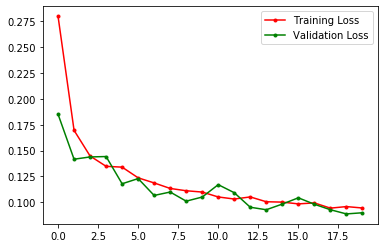
\includegraphics[width=\textwidth]{beijing-ssim-training}
% 		\caption{Beijing SSIM}
% 		\label{fig:beijing-ssim-training}
% 	\end{subfigure}
% 	\hfill
% 	\begin{subfigure}[b]{0.7\textwidth}
% 		\centering
% 		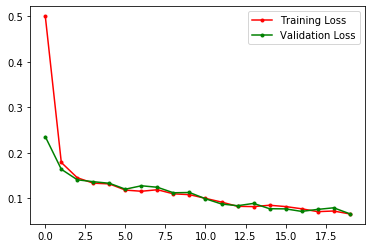
\includegraphics[width=\textwidth]{shanghai-ssim-training}
% 		\caption{Shanghai SSIM}
% 		\label{fig:shanghai-ssim-training}
% 	\end{subfigure}
% 	\hfill
% 	\begin{subfigure}[b]{0.7\textwidth}
% 		\centering
% 		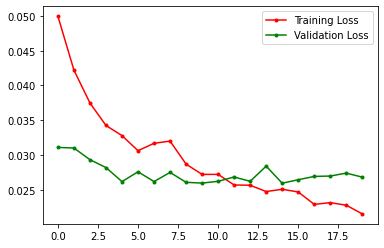
\includegraphics[width=\textwidth]{shanghai-ssim-transfer-learning}
% 		\caption{Shanghai SSIM Transfer Learning}
% 		\label{fig:shanghai-ssim-transfer-learning}
% 	\end{subfigure}
% 	\caption{Comparision of loss graph in applying transfer learning in SSIM}
% 	\label{fig:}
% \end{figure}


\begin{table}[h]
\centering
\begin{tabular}[widht=\textwidth]{|l | l | l | l | l|}
\hline
 & Beijing data & Shanghai data  & Shanghai with TL & Improvement \\
\hline
CNN & 0.0763 & 0.031 & 0.015 & 52 \% \\

SSIM & 0.0944 & 0.0656 & 0.0215 & 67 \% \\
\hline
\end{tabular}
\caption{Comparision of MSE Loss of various model with transfer learning}
\label{tab:comparision-table}
\end{table}


\textbf{MSE Loss}
MSE (Mean Squared Error) is the loss function that is used for the training the models on the sensor data. It is used to measure the efficienty of the model trained. Lesser the value of MSE score more the model is efficient. \\

\begin{figure}[ht]
	\centering
	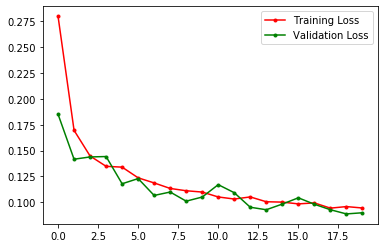
\includegraphics[width=0.8\textwidth]{beijing-ssim-training}
	\caption{Beijing SSIM}
	\label{fig:beijing-ssim-training}
\end{figure}


\textbf{Beijing data on CNN model}
On training CNN model with bejing data mse score achived is 0.763 \\

\textbf{Beijing data on SSIM model}
On training SSIM model with beijing data mse score achieved is 0.0944 \\

This results that SSIM model achieved more efficiency in comparision to CNN model for time series frecasting problem.\\



\begin{figure}[ht]
	\centering
	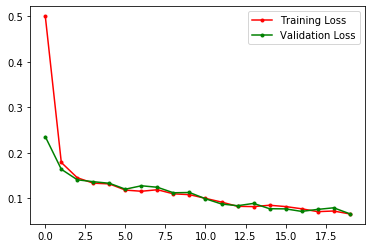
\includegraphics[width=0.8\textwidth]{shanghai-ssim-training}
	\caption{Shanghai SSIM}
	\label{fig:shanghai-ssim-training}
\end{figure}

\textbf{Shanghai data on SSIM without Transfer Learning}
On training SSIM model with shanghai data without Transfer learning mse score achieved is 0.0656\\

\textbf{Shanghai data on SSIM with Transfer Learning}
On training SSIM model with shanghai data with Transfer learning with using pretrained model of beijing data mse score achieved is 0.0215 \\

\begin{figure}[ht]
	\centering
	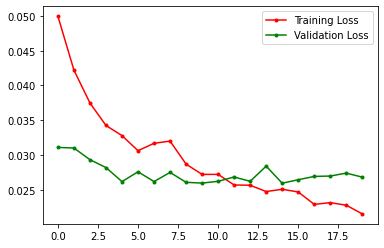
\includegraphics[width=0.8\textwidth]{shanghai-ssim-transfer-learning}
	\caption{Shanghai SSIM Transfer Learning}
	\label{fig:shanghai-ssim-transfer-learning}
\end{figure}


This results that SSIM model with transfer learning shows 67\% improvement. \\

Figure \ref{fig:beijing-ssim-training} shows the training vs validation loss graph of Beijing SSIM training \\

Figure \ref{fig:shanghai-ssim-training} show the training vs validation loss graph of Shanghai SSIM training \\

Figure \ref{fig:shanghai-ssim-transfer-learning} shows the training vs validation loss graph of Shanghai SSIM training with transfer learning with using pretrained bejing ssim model. \\

Table \ref{tab:comparision-table} Summarises all the models losses and imporvements. \\

While using SSIM model there is 67\% imporvement with transfer learning.\\

Also\\

While using CNN model there is 52\% improvement with transfer learning. \\






